
\documentclass{article}
\usepackage[utf8]{inputenc}
\usepackage{biblatex}
\usepackage{graphicx}
\addbibresource{PQL.bib}
\usepackage{setspace}
\doublespacing
\setlength{\parskip}{1em}
\usepackage [autostyle, english = american]{csquotes}
\usepackage{amsmath}

\begin{document}

\title{Bias Induced By Fitting GLMMs with Dichotomous Outcomes Using Penalized Quasi-Likelihood}
\author{Joshua Nugent, Bianca Doone, Ken Kleinman}
\date{2019}

%\maketitle

Title: Bias Induced By Fitting GLMMs with Dichotomous Outcomes Using Penalized Quasi-Likelihood

Short Title: PQL Bias With Dichotomous Outcomes

Authors: Joshua Nugent, Bianca Doone, Ken Kleinman, (all: affiliation: Department of Biostatistics and Epidemiology, University of Massachusetts Amherst, Amherst, MA, USA)

Corresponding Author:
Ken Kleinman, 415 Arnold House, School of Public Health and Health Sciences, University of Massachusetts, 715 North Pleasant Street, Amherst, MA 01003-9304

Telephone: 413-320-6667

jnugent@umass.edu

Grant Support: NIGMS: R01 GM121370

Word Count: 2,671

Date: March 2019

\newpage

Abstract: Generalized linear mixed models (GLMMs) are the most widely-used method for analyzing data from cluster-randomized trials (CRTs). Popular statistical software packages allow for different GLMM fitting algorithms, but one of these algorithms, penalized quasi-likelihood (PQL), has been shown to produce biased parameter estimates. We review the literature to assess how widely PQL may be used, and conduct a literature-informed simulation study to show the extent of the PQL bias in plausible CRT settings. We find that the algorithms employed are rarely reported in the literature, and that PQL bias is most extreme when the cluster size is small and the variability between clusters is large. Further, intraclass correlation coefficient (ICC) estimates from PQL-fitted models are also shown to vary by outcome prevalence and treatment effect. Alternatives to PQL estimation are demonstrated to be unbiased and feasible for most CRT data analysis needs.  Analysts should not use PQL and should report fitting methods when reporting trial results.


Keywords: Cluster randomized trials, generalized linear mixed models, penalized quasi-likelihood, PQL

\newpage

\begin{flushleft}
\section{Background / Aims}

Generalized linear mixed models (GLMMs) are the most commonly used correct method for analyzing data from cluster randomized trials (CRTs). 

JN-- Is this something we can cite, or is it a something we establish here?  If the former, add a cite.  If the latter, I think we can just say "are a commonly used"

GLMMs extend generalized linear models (GLMs) by including an additional random-effects term in the linear predictor. This term captures variance between clusters - for example, the group-level differences between hospitals or classrooms. In settings where interventions are applied at the cluster level, GLMMs can disaggregate treatment effects from any preexisting underlying variance between clusters. In medical settings, CRTs with dichotomous outcomes are very common - for example, estimating the effect of a new infection control protocol on MRSA incidence, or the probability of a preterm birth for people enrolled in prenatal support groups - and GLMMs are a commonly-used tool for analysis. 


The optimization problem of fitting a GLMM to data is a non-trivial task. Three common numerical methods for estimating the coefficients are \textit{penalized quasi-likelihood} (PQL), \textit{Gauss-Hermite quadrature} (GHQ), and \textit{Laplace approximation}. Other methods, such as Newton quadrature, Monte Carlo integration, and Markov Chain Monte Carlo can be used as well \cite{zhang_fitting_2011}, but since popular statistical software packages use PQL, GHQ, and Laplace approximation as their standard GLMM fitting algorithms, we will focus on those in this paper. The full mathematical details of these three main methods have been elaborated in other sources \cite{wolfinger_generalized_1993}\cite{pinheiro_efficient_2006}, and an overview of the technical aspects of GLMMs and the algorithms is given in the Appendix.

JN-- I deleted the end of a sentence above that explained that we would not focus on what was "under the hood".  In general, I try to avoid colloquial and idiomatic expressions in scientific writing, but it's possible that I'm an old fuddy-duddy.


Penalized quasi-likelihood was popularized by Breslow and Clayton\cite{breslow_approximate_1993}, though similar methods were developed by others\cite{zeger_models_1988}\cite{engel_simple_1994} around the same time. Though it is computationally efficient, especially for models with many random effects, PQL can induce bias in certain cases, in particular when the response variable distribution is far from normal\cite{agresti_categorical_2013}\cite{rodriguez_assessment_1995}\cite{breslow_bias_1995}\cite{lin_bias_1996}. Additionally, PQL produces Wald-type test statistics, not true likelihoods, making it unsuitable for use in the likelihood ratio test.  Thus is cannot be used in nested model selection\cite{zhang_fitting_2011}\cite{pinheiro_efficient_2006}\cite{ng_estimation_2006}.

Gauss-Hermite quadrature is a more computationally demanding method, but shows no discernible bias, and can produce true likelihood statistics for model comparison. The accuracy with which it computes the model fit is a function of how many \textit{quadrature points} it uses in estimating the model. All else being equal, the computation time is roughly proportional to $(N_q)^u$, where $N_q$ is the number of quadrature points and $u$ is the number of random effects at all levels of the model \cite{statacorp_stata_2017}\cite{pinheiro_efficient_2006}. For a model with 4 random effects and 5 quadrature points, $(N_q)^u = 5^4 = 625$. Doubling the number of points to 10 changes that result to $10,000$, a factor of 16. For data sets with large numbers of random effects, this can limit the utility of GHQ.

JN-- please edit the para above to avoid the suggestion that GHQ has a mind of its own

Luckily for the data analyst, many CRTs have only one random effect, so computation time will increase linearly with the number of quadrature points, rather than as a power function. Furthermore, if many models need to be compared, using one quadrature point can give preliminary results rapidly. Then, after that model selection process, the number of quadrature points can be increased to make the final estimates as accurate as computationally possible. Empirical results suggest that 7 or fewer quadrature points often give suitably accurate estimates\cite{pinheiro_approximations_1995}.

Laplace approximation is equivalent to GHQ with a single quadrature point\cite{liu_note_1994}, and as such it produces true likelihoods for model comparison. While its accuracy is typically lower than GHQ with $N_q\geq2$, under certain circumstances it performs quite well\cite{liu_note_1994}.

For reasons of computational efficiency, PQL was a useful method for fitting GLMMs when it was developed, but with the advent of more modern computers, less biased methods such as GHQ have become an attractive alternative. For CRTs with binary outcomes, where the bias in PQL is the most extreme\cite{ng_estimation_2006}\cite{lin_estimation_2007}, and where the presence of only one random effect is typical, using GHQ is the best option: fast enough, and, more importantly, unbiased.

Most modern statistical software packages have functions to fit GLMMs with dichotomous outcomes, such as PROC GLIMMIX in SAS, meglm in Stata, and glmer (from the lme4 package, as well as others) in R. However, the default fitting algorithm in each of those functions varies. In SAS PROC GLIMMIX, the default is PQL, with Laplace or GHQ available if specified. In R, the glmer function default is Laplace, with GHQ available if specified; PQL is only available in R via the glmmPQL function in the MASS package. In Stata, meglm defaults to GHQ with 7 quadrature points, with Laplace available if specified.

Given that many data analysts may be unfamiliar with the fitting options, a function's default settings are influential in the final results. Below, we investigate how often functions and algorithms are reported in the literature and use simulations to describe the bias induced by PQL in a literature-informed, plausible CRT scenario.




\section{Methods}

We started by conducting a literature review among recent CRTs with dichotomous outcomes to determine a) common values for cluster size and number of clusters and b) what software, functions, and fitting algorithms were used to analyze the data, if reported. The review, searching for the phrase "cluster randomized trial" in the title or abstract of the article, spanned two databases over two timeframes. First, we searched the The New England Journal of Medicine, The British Medical Journal, The Journal of the American Medical Association, and The Lancet from January 1, 2014 through August 31, 2018, using the Web of Science database. Second, we did a broader search of all articles in the PubMed database published between March 1st, 2018 and August 31, 2018. 

Having identified candidate articles, we filtered to completed CRTs with dichotomous outcomes. The mean number of observations per cluster and number of clusters for each study was recorded, as well as the software and functions/algorithms the authors used, if available.


JN-- revise paras above to refer to the brief note we just submitted.  This might be just adding a sentence to say that futher details are available there??  


The second phase of our work was a simulation study to investigate the bias of different GLMM fitting algorithms for dichotomous outcomes. To maximize the utility of the results, our simulations used a range of plausible cluster counts and cluster sizes drawn from the literature review.

Our data-generating mechanism for the simulations was a simple logistic-link GLMM with one fixed intercept, one treatment effect, and one random intercept, defined as:
\begin{equation}
    \text{logit}[\pi(y_{ij}|u_j)]=\beta_0 + \beta_1 x_{ij} + b_j
\end{equation}
with $x_{ij}$ an indicator for treatment (1) or control (0) arm of the study for observation $i$ in cluster $j$; $\pi(y_{ij}|b_j)$ the probability of the outcome for individual $i$ in cluster $j$; $e^{\beta_0}$ the baseline odds of the outcome across all clusters; $e^{b_j}$ the odds ratio compared to baseline for the outcome, specific to observations in cluster $j$ relative to the mean cluster, with assumed distribution $b_j \sim N(0, \sigma_{0}^2)$; and $\beta_1$, our parameter of interest, the log odds ratio due to the treatment. 

JN-- why not just have $Pr(y_ij|b_j) = 1)$, instead of $\pi(y_ij|b_j)$ on the LHS?  Also, in either case, you have to also describe what $y_ij$ means.  Also aso, why not just $\sigma^2$, instead of $\sigma^2_0$?


From that model, populations were generated with the following parameter values, informed by the literature review (see Table \ref{tab:lit_review_numbers}):
\begin{itemize}
    \item Number of clusters $n \in \{10, 50, 100\}$
    \item Number of observations per cluster $p \in \{25, 100\}$
    \item $\beta_0$ values corresponding to a baseline prevalence of .01, .02, .03, .05, .1, and .2
    \item $\beta_1$ values corresponding to a treatment effect odds ratio of .5, .75, .9, 1.1, 1.33, 1.5, and 2
    \item $\sigma^2_0$ values of 1 (high cluster variability) and .1 (low cluster variability).
\end{itemize}

Using 3000 simulated populations for each combination of parameters, logistic-link GLMMs were fit via PQL, GHQ, and Laplace using SAS software version 9.4 (SAS Institute, Cary, NC).

JN-- populations?  Maybe trials?

The distribution of $\hat{\beta_1}$ estimates from each method was compared to the true value from the data-generating mechanism and absolute bias was measured as the difference between the two. The standard errors of estimates and the estimated cluster variance ($\hat{\sigma}^2_0$) were also collected from the fitted models. Finally, the simulated populations were re-fit under the assumption that the outcome variable was normally distributed, without the logit link, and the intraclass correlation coefficient (ICC) estimated from those models was collected.




\section{Results}

Results of the literature review are shown in Table~\ref{tab:lit_review}. Of the 85 articles, only 9 identified the specific procedure (meglm or GLIMMIX, for example) used. Among the 24 articles that identified SAS as one of the software packages, only 3 specified which SAS procedure was used and only one identified the model fitting algorithm.

\begin{table}[]
\centering
Software cited (specific procedures or functions)
 \begin{tabular}{ |l||c|c|c|c|c| } 
 \hline
      & R & SAS & SPSS & Stata & Unreported\\ 
     \hline
    Top4 2014 - 2018 ($n=42$) & 11 (2) & 13 (1) & 2 (0) & 18 (2) & 4 (4)  \\ 
    PubMed Q2 2018 ($n=43$) & 3 (0) & 11 (2) & 8 (0) & 14 (2) & 10 (0) \\ 
    \hline
    Total ($n=85$) & 14 (2) & 24 (3) & 10 (0) & 32 (4) & 14 (0) \\ 
\hline
 \end{tabular}
    \caption{Cited software used for data analysis. Numbers in parentheses indicate number of references to specific functions or fitting options within the software package. Some articles used multiple software packages, so the totals differ from $n$. While most articles report the software used, very few of them specifically reference the function or fitting algorithm.}
    \label{tab:lit_review}
\end{table}

Parameters for the simulations were chosen after observing the common values in Table~\ref{tab:lit_review_numbers}. The number of clusters was typically below 100, as was the number of observations per cluster, though the latter showed significantly more variability.

\begin{table}[]
\centering
 \begin{tabular}{ |l||c|c| } 
 \hline
      & Median number of & Median observations per \\ 
      & clusters (middle 50\%) & cluster (middle 50\%) \\ 
     \hline
    Top4 2014 - 2018 ($n=42$) & 46 (24 - 116) & 110 (40 - 487) \\ 
    PubMed Q2 2018 ($n=43$) & 32 (15 - 70) & 44 (14 - 205) \\ 
    \hline
    Total ($n=85$) & 40 (16 - 90) & 66 (19 - 300) \\
    \hline
 \end{tabular}
    \caption{Common values for $p$ and $n$ from the literature review.}
    \label{tab:lit_review_numbers}
\end{table}



\begin{figure}[]
\begin{center}
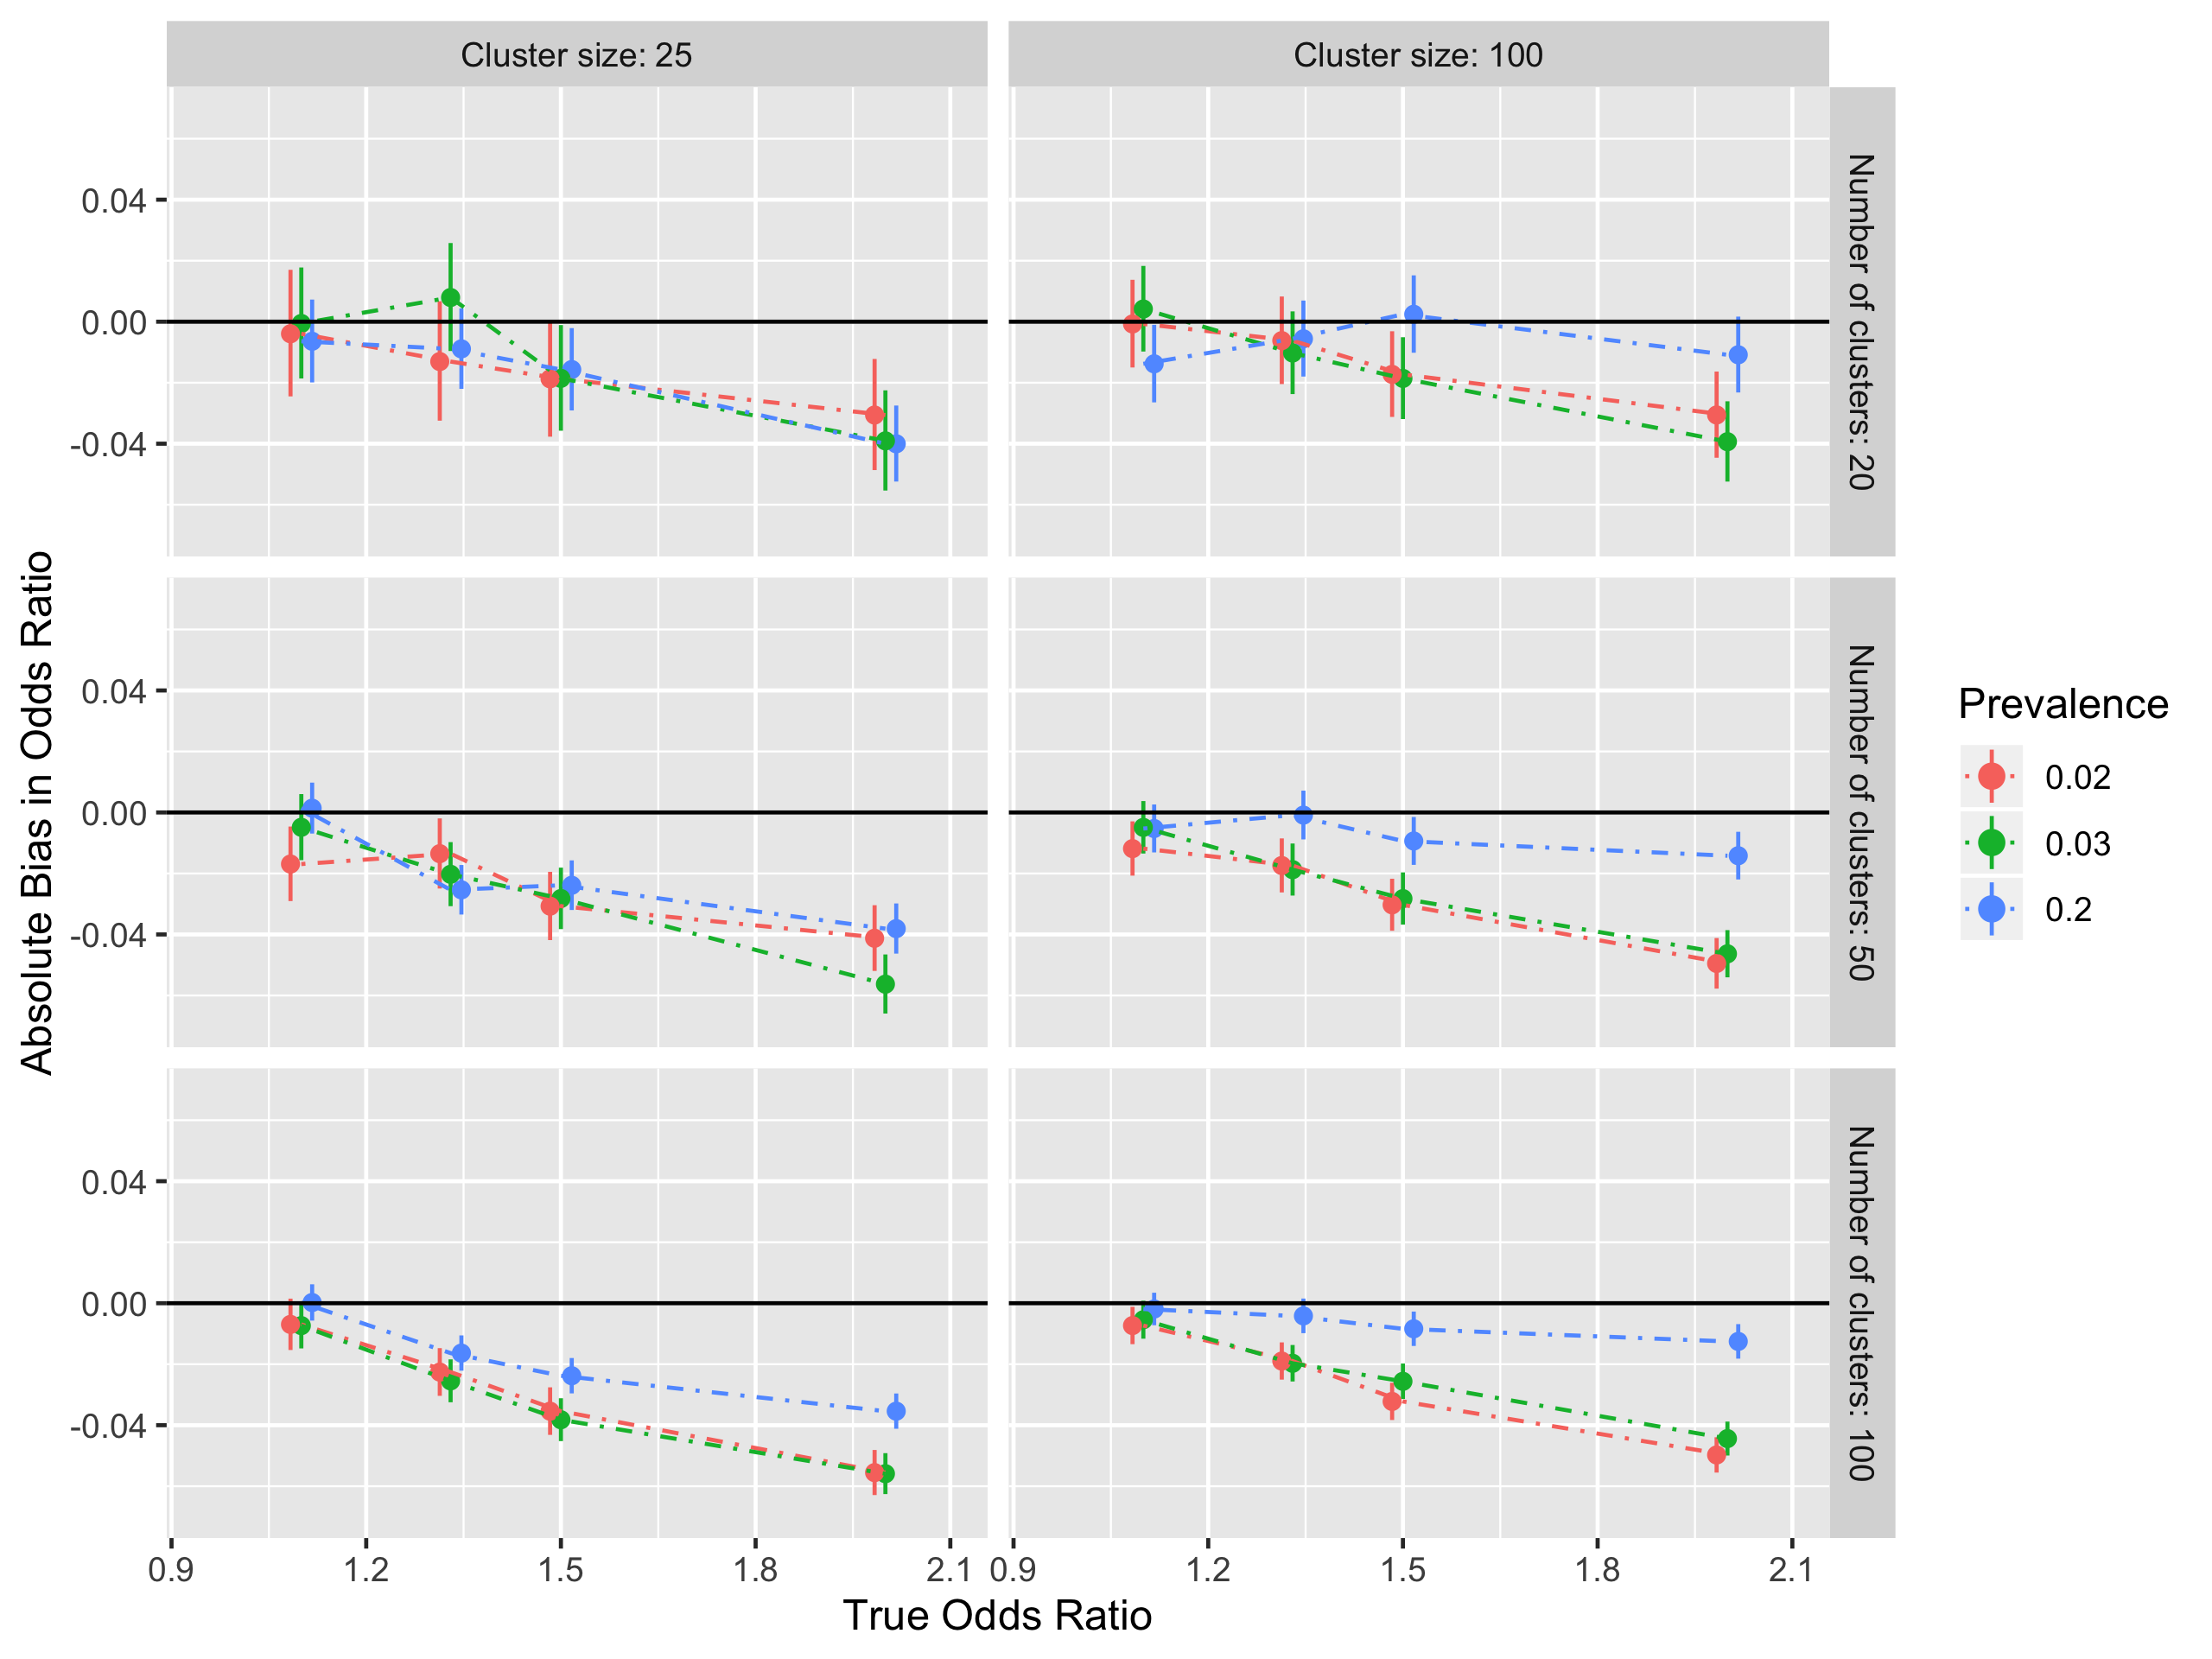
\includegraphics[width=\textwidth]{_bias_pql_sbs1.png}
  \caption{Odds ratio bias ($\text{exp} \{ \bar{\hat{\beta_1}} - \beta_1 \}-1$) in PQL estimation, $\sigma^2_0=1$, cluster size $p$, number of clusters $n$. Simulation runs with less than 80\% convergence omitted. Note larger scale in the first row.}
    \label{fig:_bias_pql_6}
\end{center}
\end{figure}

\begin{figure}[]
\begin{center}
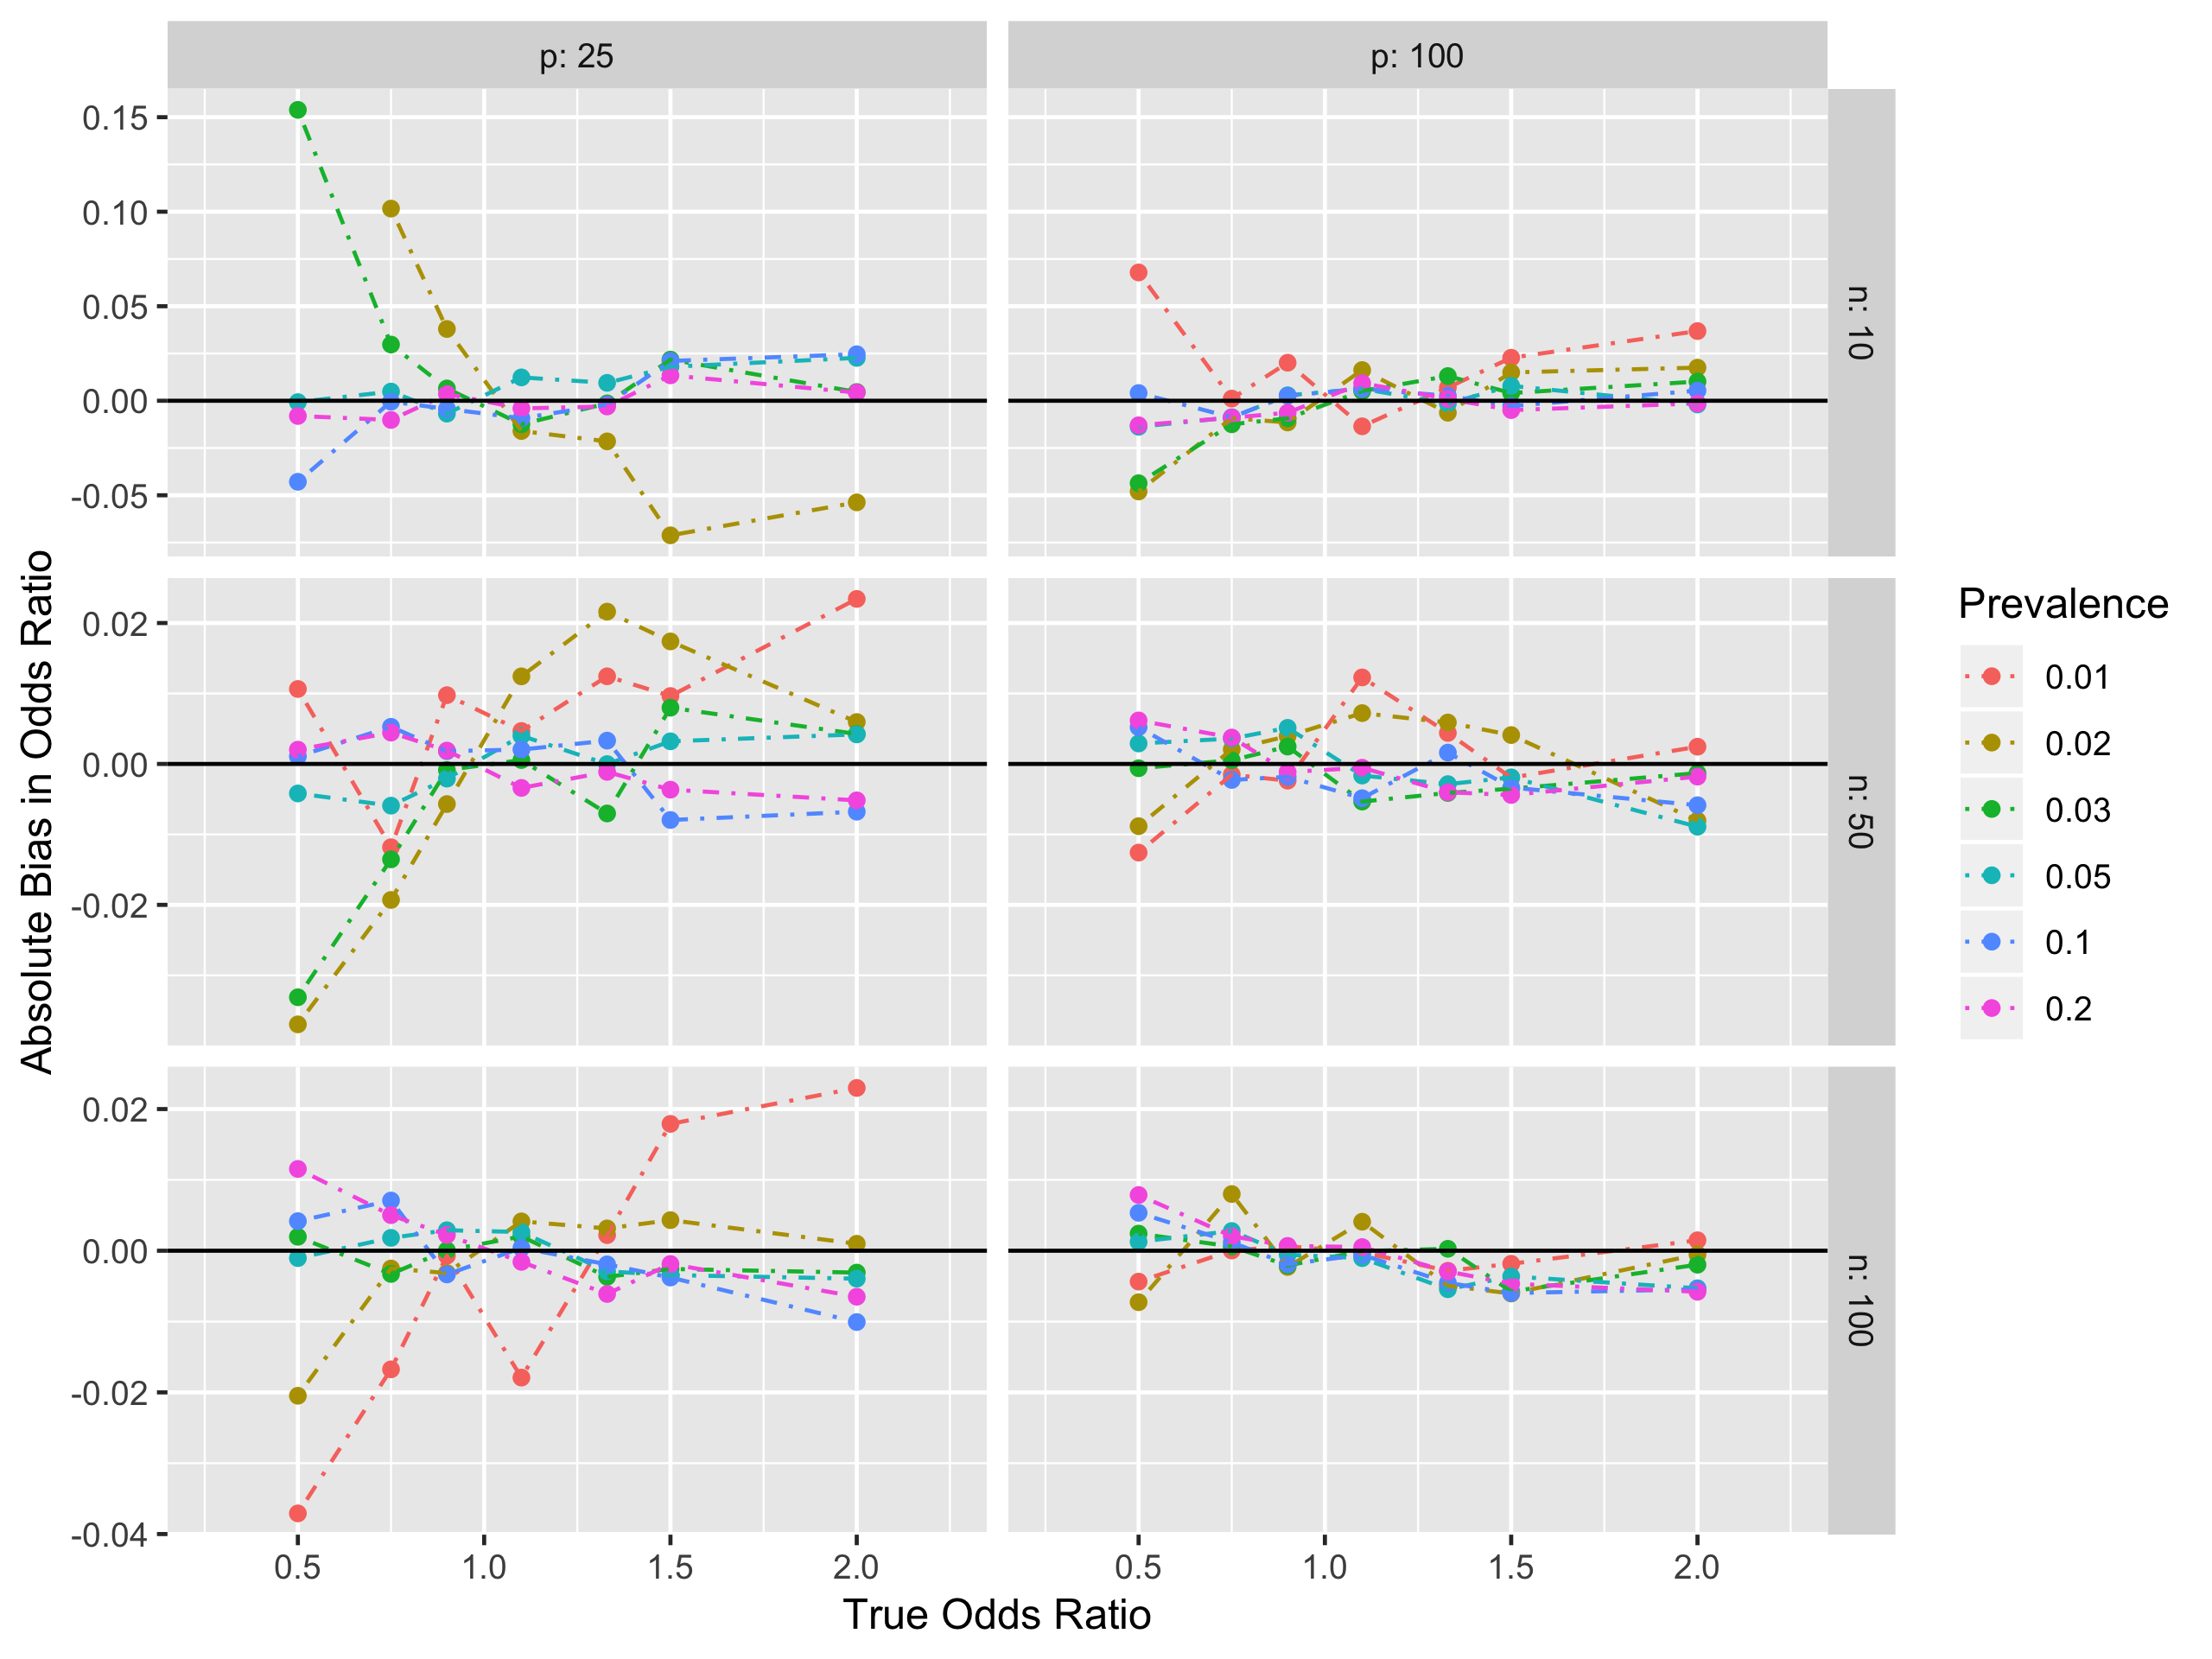
\includegraphics[width=\textwidth]{_bias_pql_sbspt1.png}
  \caption{Odds ratio bias ($\text{exp} \{ \bar{\hat{\beta_1}} - \beta_1 \} - 1$) in PQL estimation, $\sigma^2_0=0.1$, cluster size $p$, number of clusters $n$. Simulation runs with less than 80\% convergence omitted.}
    \label{fig:_bias_pql_sbs_pt1}
\end{center}
\end{figure}

\begin{figure}[]
\begin{center}
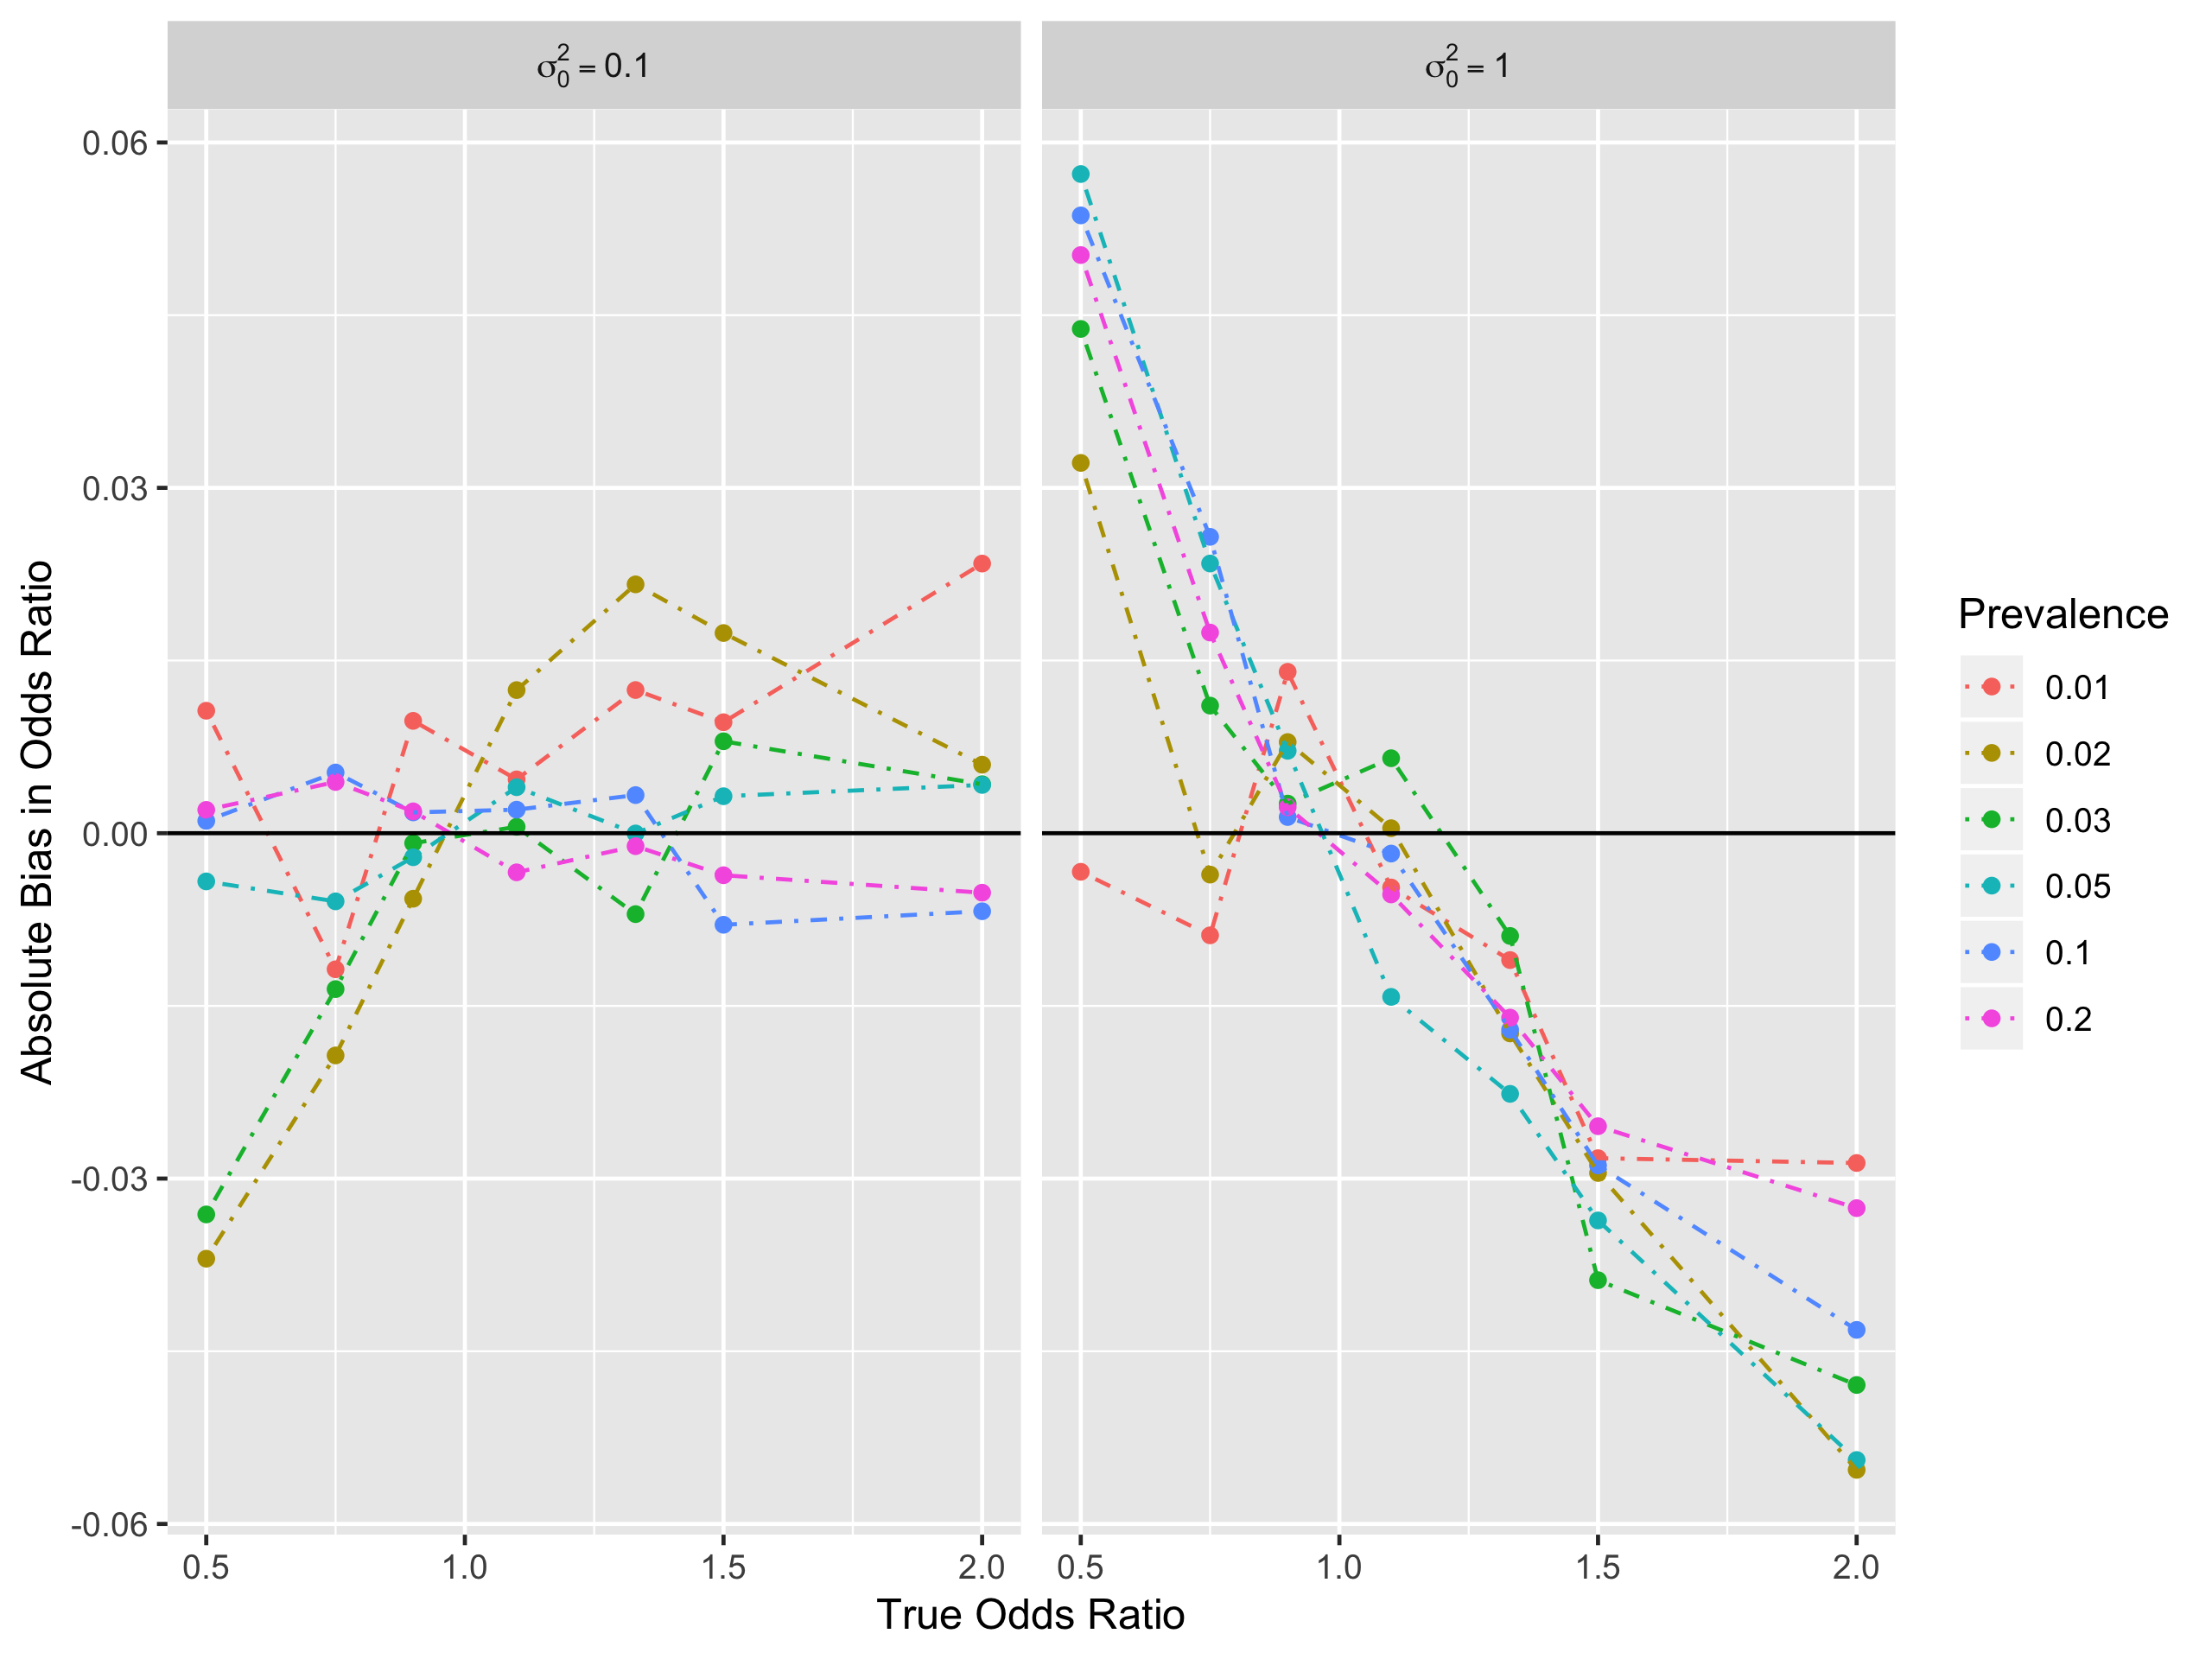
\includegraphics[width=\textwidth]{_bias_pql_sbs_p25_n50.png}
  \caption{Odds ratio bias ($\text{exp} \{ \bar{\hat{\beta_1}} - \beta_1 \}-1$) in PQL estimation for different $\sigma^2_0$, $p=25$, $n=50$.}
    \label{fig:_bias_pql_sbs_single_comparison}
\end{center}
\end{figure}

JN-- let's make sure to talk about convergence issues.


The results of the bias investigation in PQL estimation are shown in Figures \ref{fig:_bias_pql_6}-\ref{fig:_bias_pql_sbs_single_comparison}. The results show bias towards the null: As the true odds ratio rises above 1, there is a negative bias, meaning the mean estimated odds ratio is closer to 1 than it should be. When the odds ratio is less than one, conversely, there a positive bias towards 1. Further, while the data are noisy, the bias is more pronounced for smaller cluster sizes and when the outcome's baseline prevalence is lowest. The bias occurs, to a differing extent, across all values of prevalence, treatment effect, cluster size, and number of clusters. Figure \ref{fig:_bias_pql_sbs_single_comparison} demonstrates that the effect of high between-cluster variability is more pronounced bias.

Further, the standard errors of the estimate for $\beta_1$ are quite large in these simulations. For example, in the setting where $p=25$,

JN-- $p = .25$, maybe??

$n=100$, and $\sigma_0^2=1$, it was not uncommon to have standard errors ten times larger than the bias. This means that even a small amount of bias on a large estimated value could pull a finding above the $p<.05$ threshold.

JN-- I don't follow the logic, here.

The fitted models using GHQ (a representative example is given in Figure \ref{fig:_bias_pql_ghq4}) and Laplace approximation (Figure \ref{fig:_bias_pql_lap}) did not show a clear bias; in each, PQL is shown for reference. In a small number of simulation runs, particularly with a small number of clusters and rare outcomes, the GHQ and Laplace algorithms became unstable, leading to estimates that tended toward infinity, making the mean bias comparison unhelpful - this can be seen in the outlier in Figure \ref{fig:_bias_pql_lap} when the prevalence is .01 and the treatment effect odds ratio is 2. On the other hand, when the number of clusters is small, the PQL algorithm was less likely to converge, implying that limited data is a challenge for all of the algorithms.

\begin{figure}[]
\begin{center}
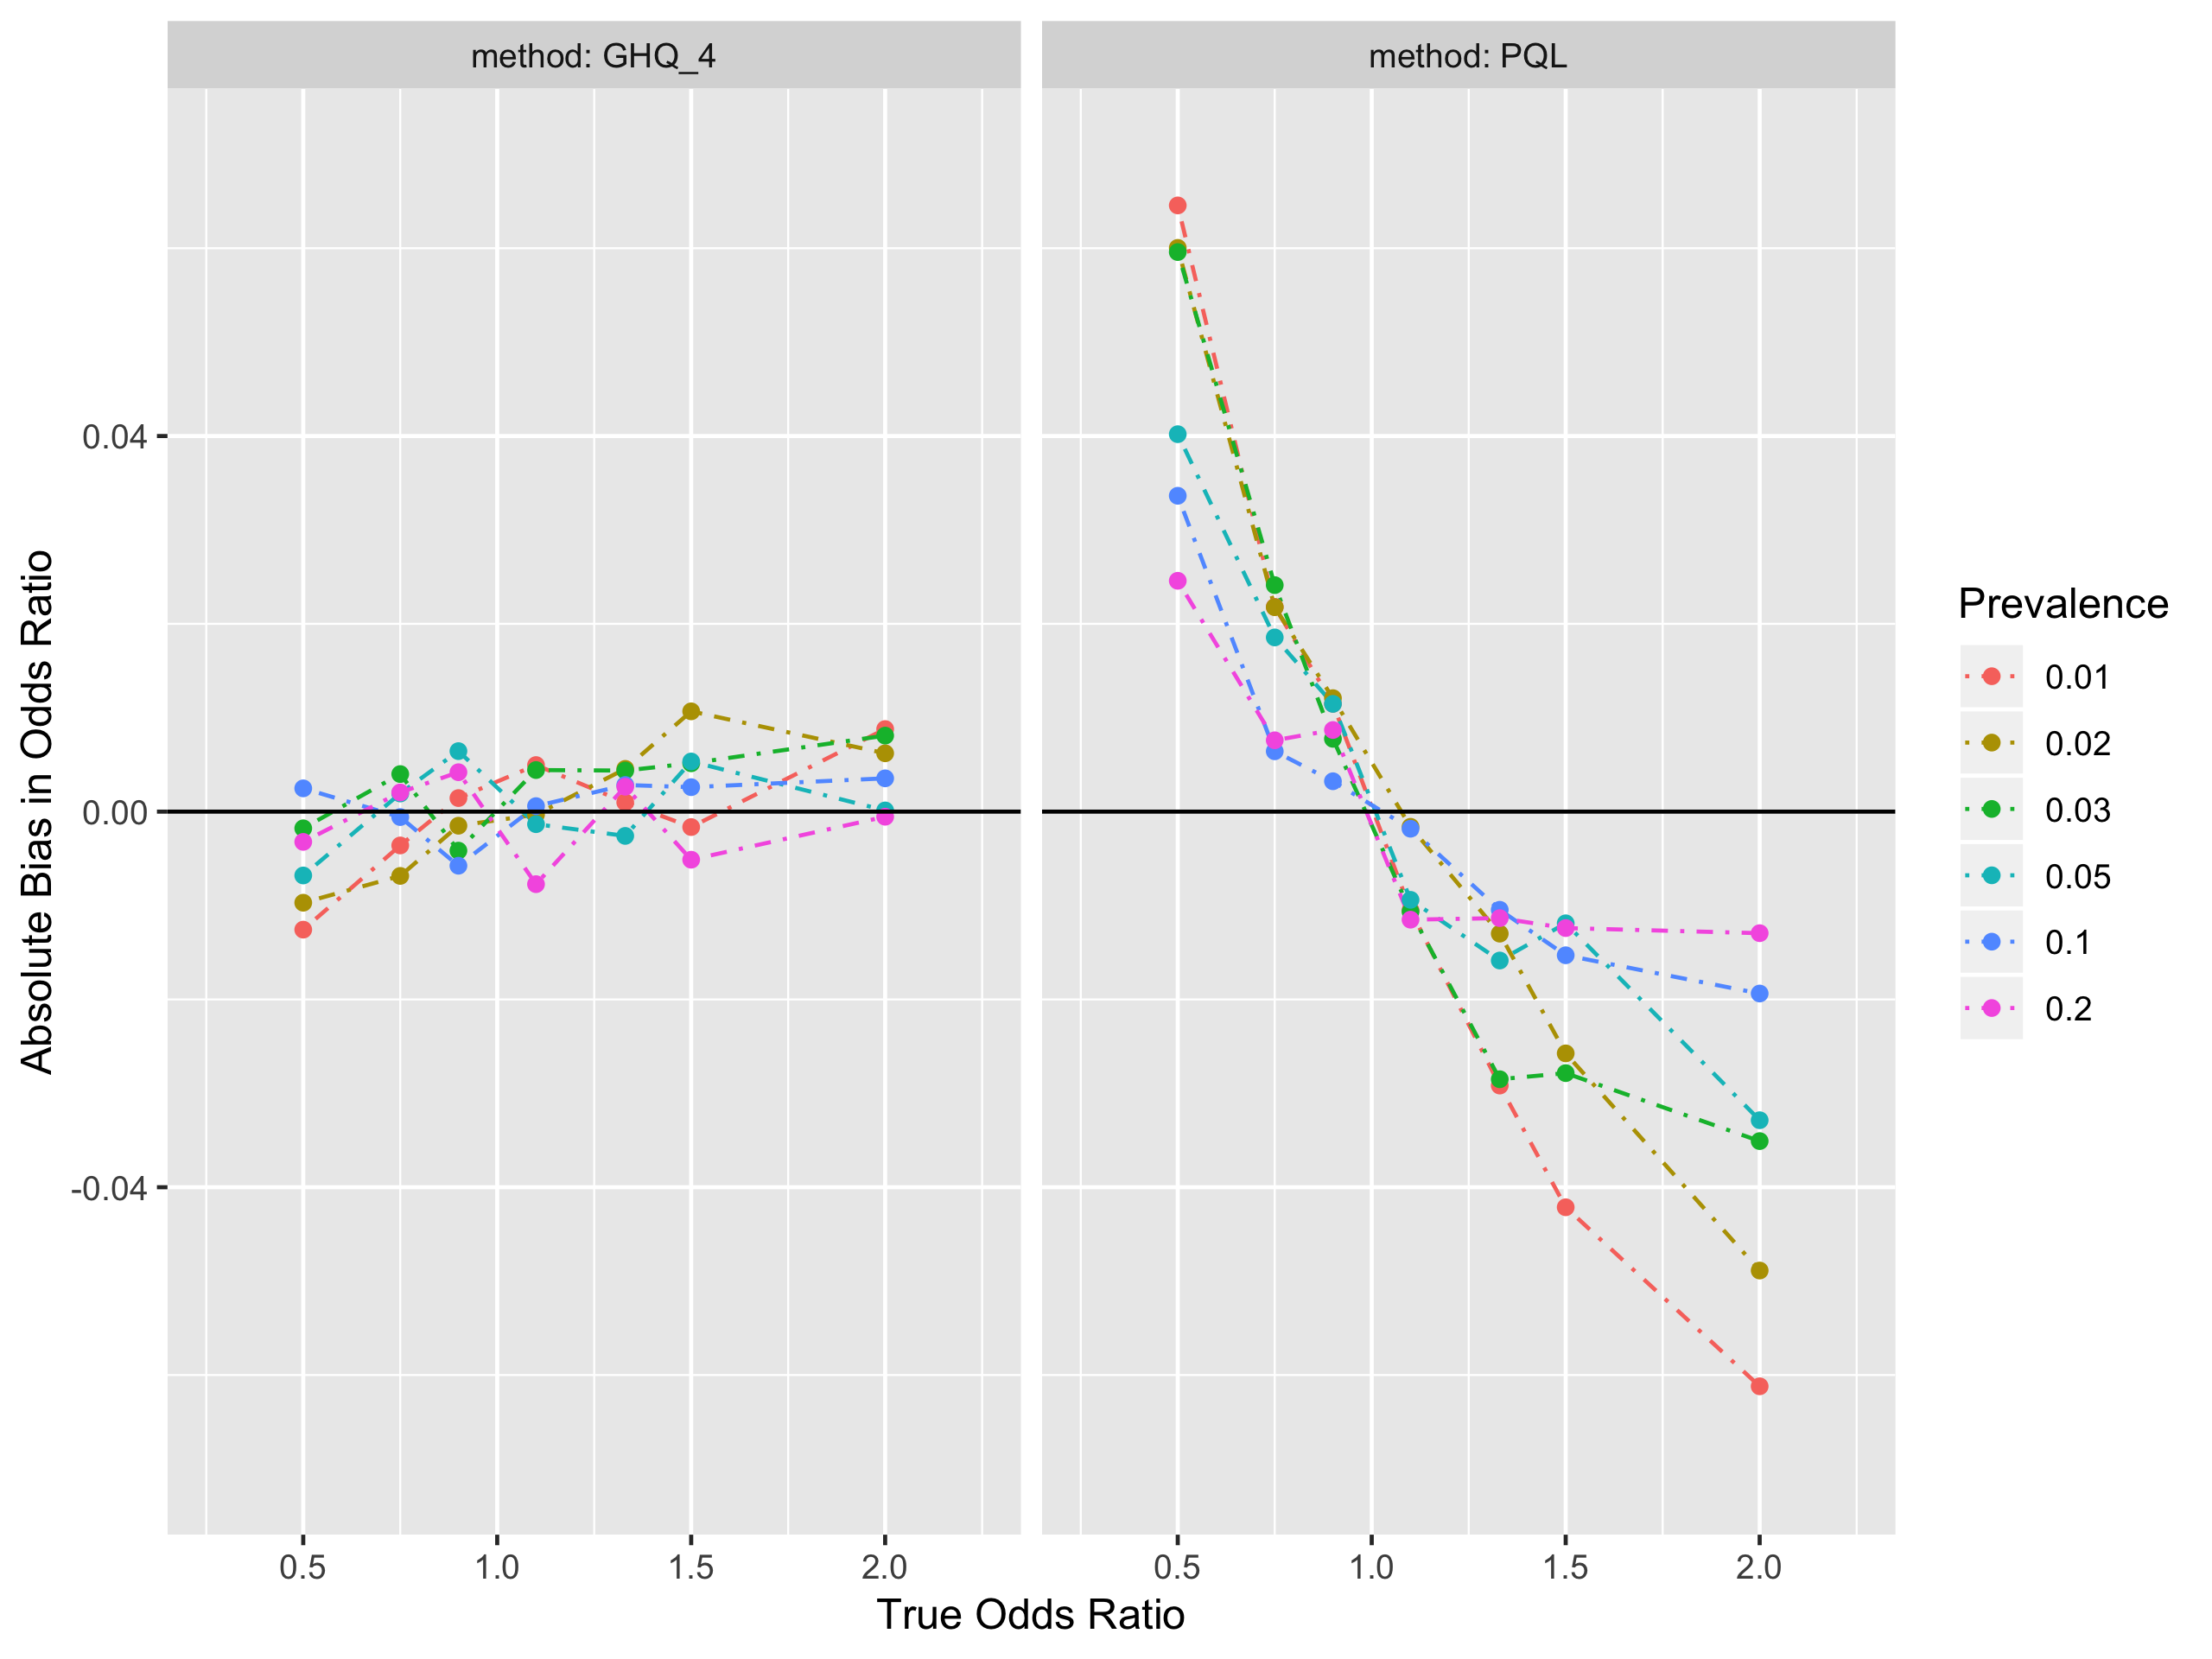
\includegraphics[width=8cm]{_bias_pql_ghq4.png}
  \caption{Odds ratio bias ($\text{exp} \{ \bar{\hat{\beta_1}} - \beta_1 \} - 1$) in GHQ (4 quadrature points) and PQL, $\sigma^2_0=1$, $p=100$, $n=100$.}
  \label{fig:_bias_pql_ghq4}
\end{center}
\end{figure}

\begin{figure}[]
\begin{center}
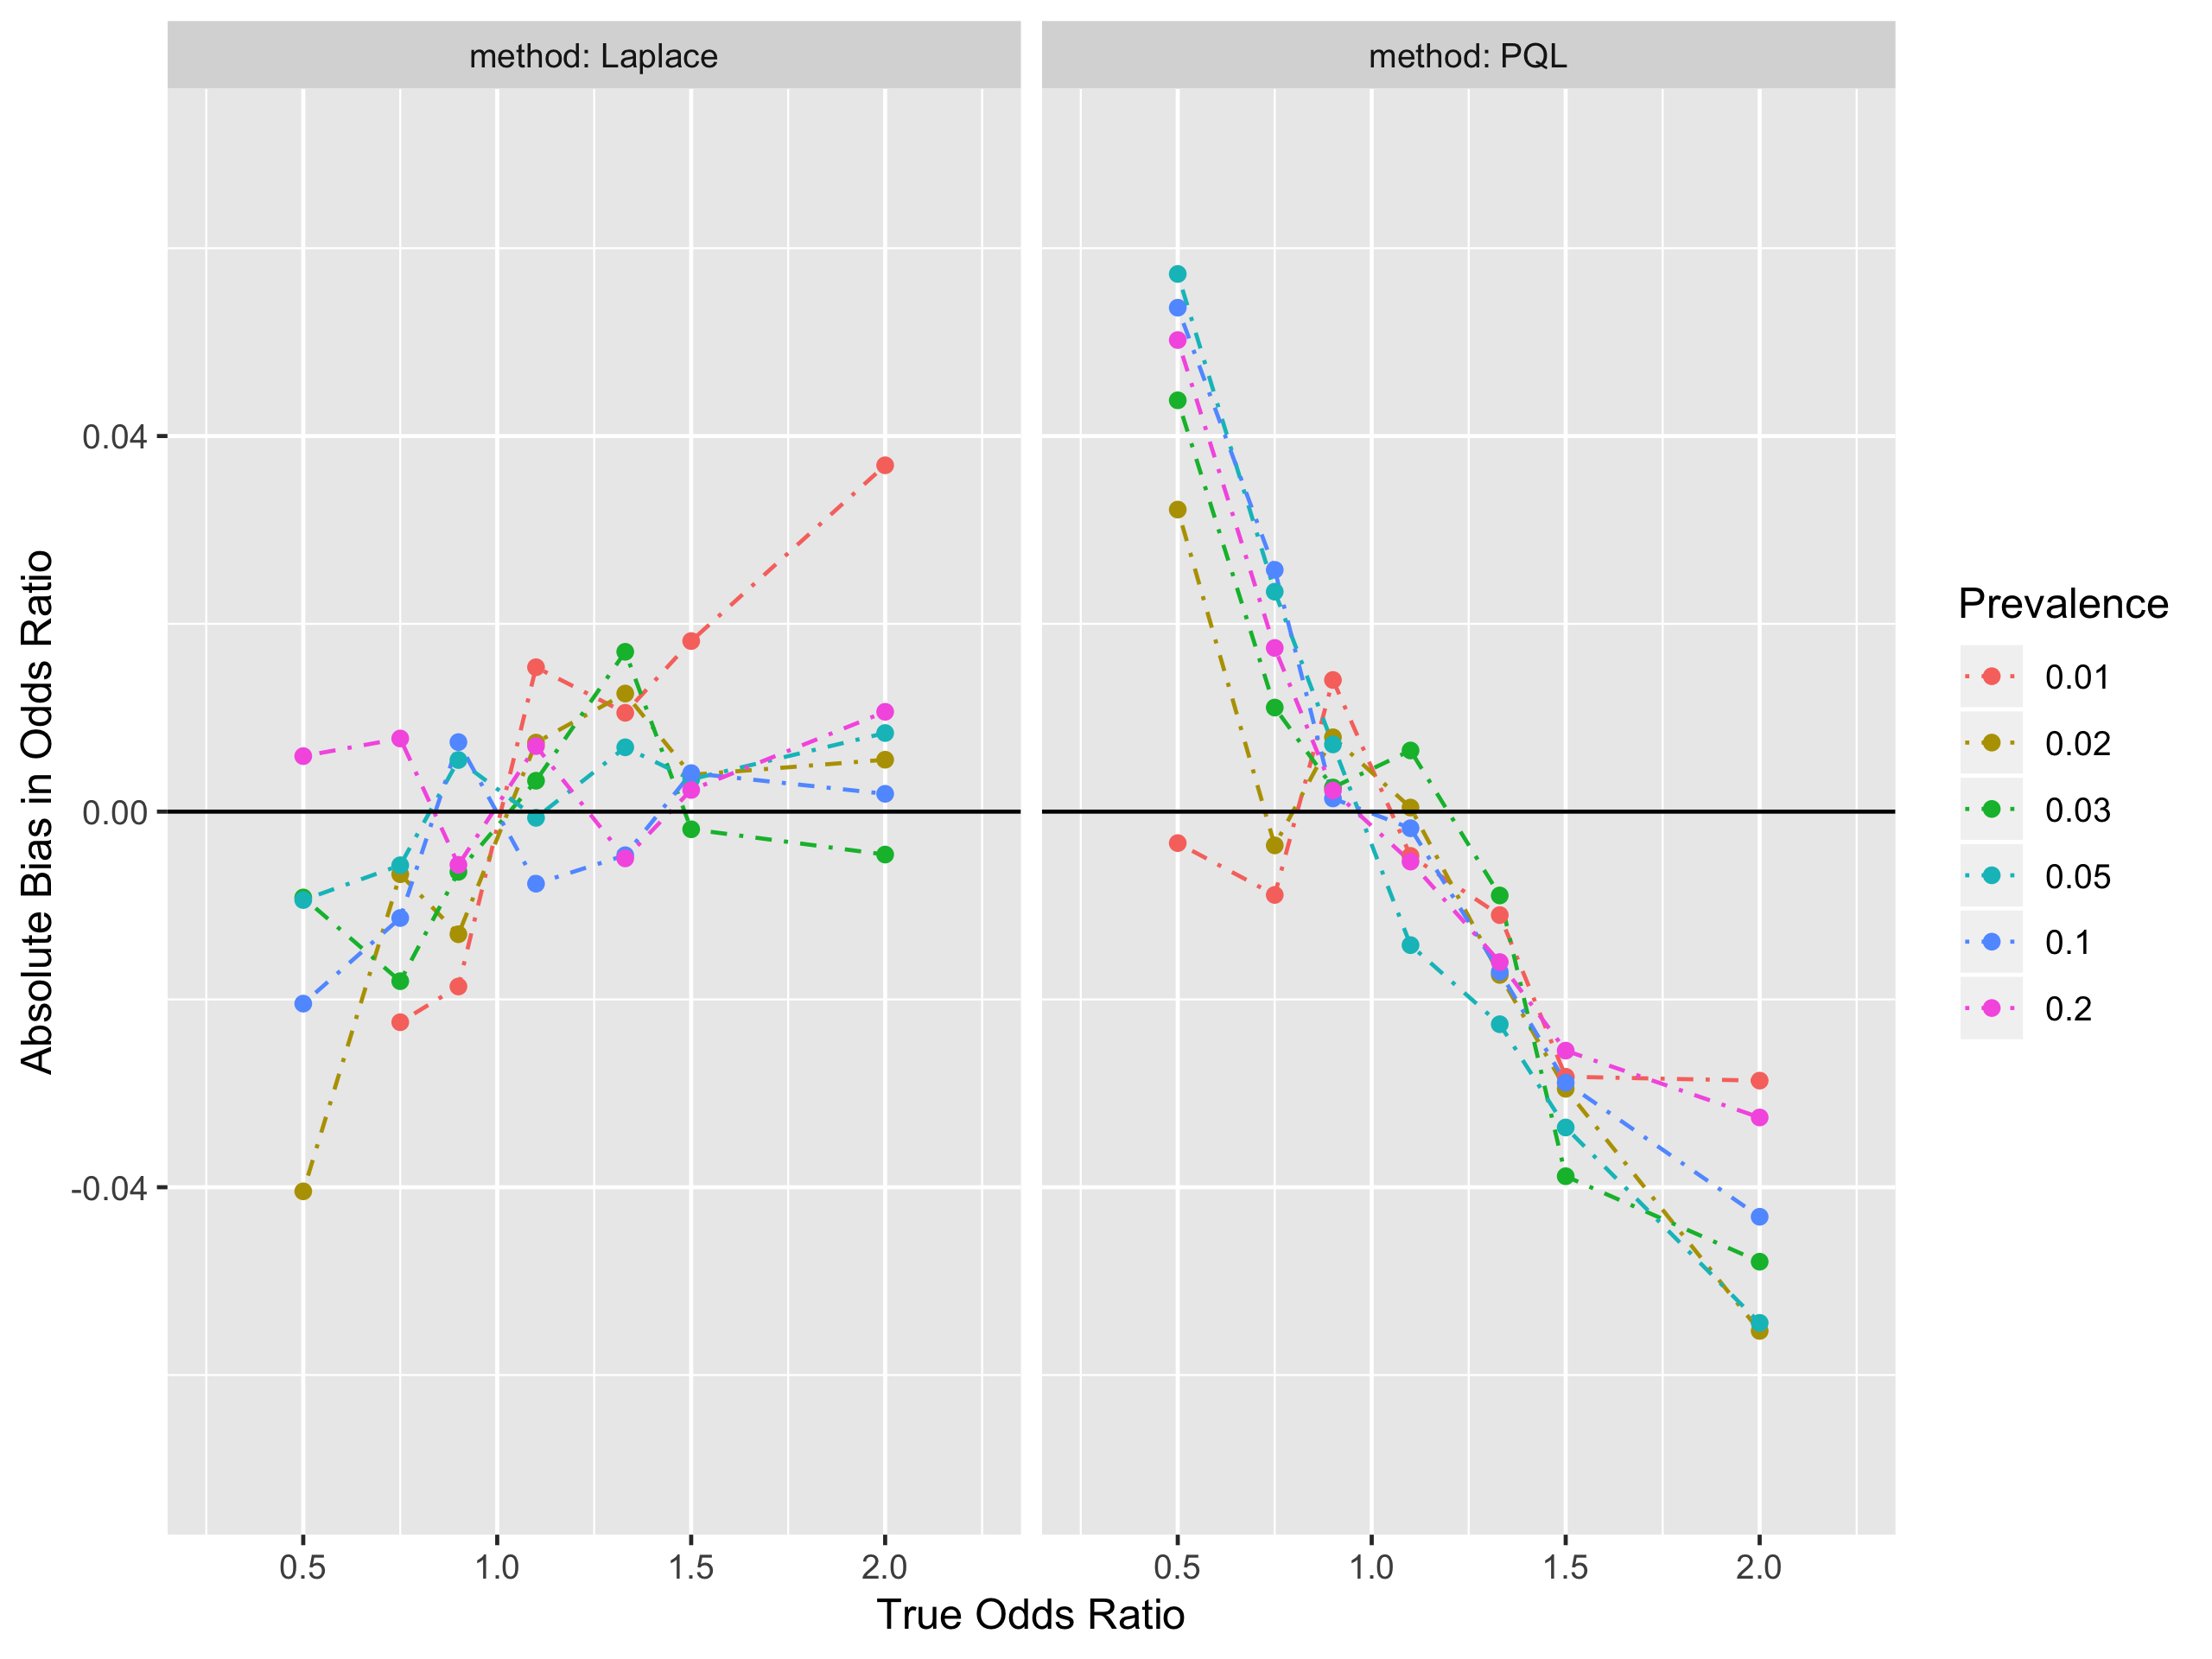
\includegraphics[width=8cm]{_bias_pql_lap.png}
  \caption{Odds ratio bias ($\text{exp} \{ \bar{\hat{\beta_1}} - \beta_1 \} - 1$) in Laplace and PQL, $\sigma^2_0=1$, $p=25$, $n=50$. Note that the lack on convergence in some of the Laplace models leads to the outlier at odds ratio 2.}
  \label{fig:_bias_pql_lap}
\end{center}
\end{figure}


JN-- following sentence belongs in the conclusion

Given the bias it creates, why use PQL? 

JN-- introduce idea that we will compare speed in the methods

Our simulations confirmed that the main advantage of using PQL over GHQ is speed.  In addition, SAS's implementation of PQL outperforms the other methods. The mean CPU time for SAS to fit a single large data set (500 clusters, 500 observations per cluster) on a modern laptop is 3.7 seconds for PQL, 11 seconds for Laplace approximation, 18.4 seconds for GHQ with $N_q=4$, and 27.1 seconds for GHQ with $N_q=10$. Results for GHQ and Laplace approximation are comparable for R's lme4 package, though the glmmPQL method from the MASS package, with a runtime of at 23.3 seconds, is significantly less efficient than in the SAS implementation. However, even for this large data set, none of the runtimes above are prohibitively long. In a situation where many models need to be tested, the Laplace method could be used to compare models, and then for the final analysis, a more accurate GHQ fit could be made with a large number of quadrature points.

%\begin{table}[h]
%\centering
% \begin{tabular}{| l | c c|} 
% \hline
% Method & R & SAS \\ 
% \hline
% PQL & 23.3 & 3.7 \\ 
% Laplace & 13.7 & 11.0  \\
% GHQ (4 quadrature points) & 16.1 &  18.4 \\
% GHQ (10 quadrature points) & 22.0 &  27.1 \\ 
% \hline
% \end{tabular}
%    \caption{Mean time (sec) to fit a single data set}
%    \label{tab:method_speed}
%\end{table}

For primarily historical reasons, analysts may be interested in the intraclass correlation coefficient (ICC), though it is not an actual parameter of the model. In normally distributed data, the ICC measures the proportion of total variance that is explained by the variance between groups. However, in the case of a non-normally distributed outcome variable, there has been considerable discussion about how to appropriately characterize and calculate the ICC\cite{wu_comparison_2012}\cite{nakagawa_shinichi_coefficient_2017}. We generated two ICC estimates using the PQL-fitted models from our simulation.  First, a version that assumed a random intercept logistic model, implying an ICC of $\frac{\sigma^2_0}{\sigma^2_0+\frac{\pi^2}{3}}$, based on the estimated between-cluster variance. Second, by fitting a linear mixed model that assumed the outcome variable was normally distributed, leading to the typical ANOVA-based calculation $\frac{\sigma^2_0}{\sigma^2_0+\sigma^2_{\epsilon}}$, where $\sigma^2_{\epsilon}$ represents the variance of the residuals. The results are shown in Figure \ref{fig:_icc} for the two values of $\sigma^2_0$ examined in out simulations. In both cases, the estimated ICC varies significantly by prevalence, treatment effect, and model class. Results when fitting the models with GHQ showed a similar pattern with the assumption of a normal distribution for the outcome, but more consistency when using the $\frac{\sigma^2_0}{\sigma^2_0+\frac{\pi^2}{3}}$ formulation. 

\begin{figure}[]
\begin{center}
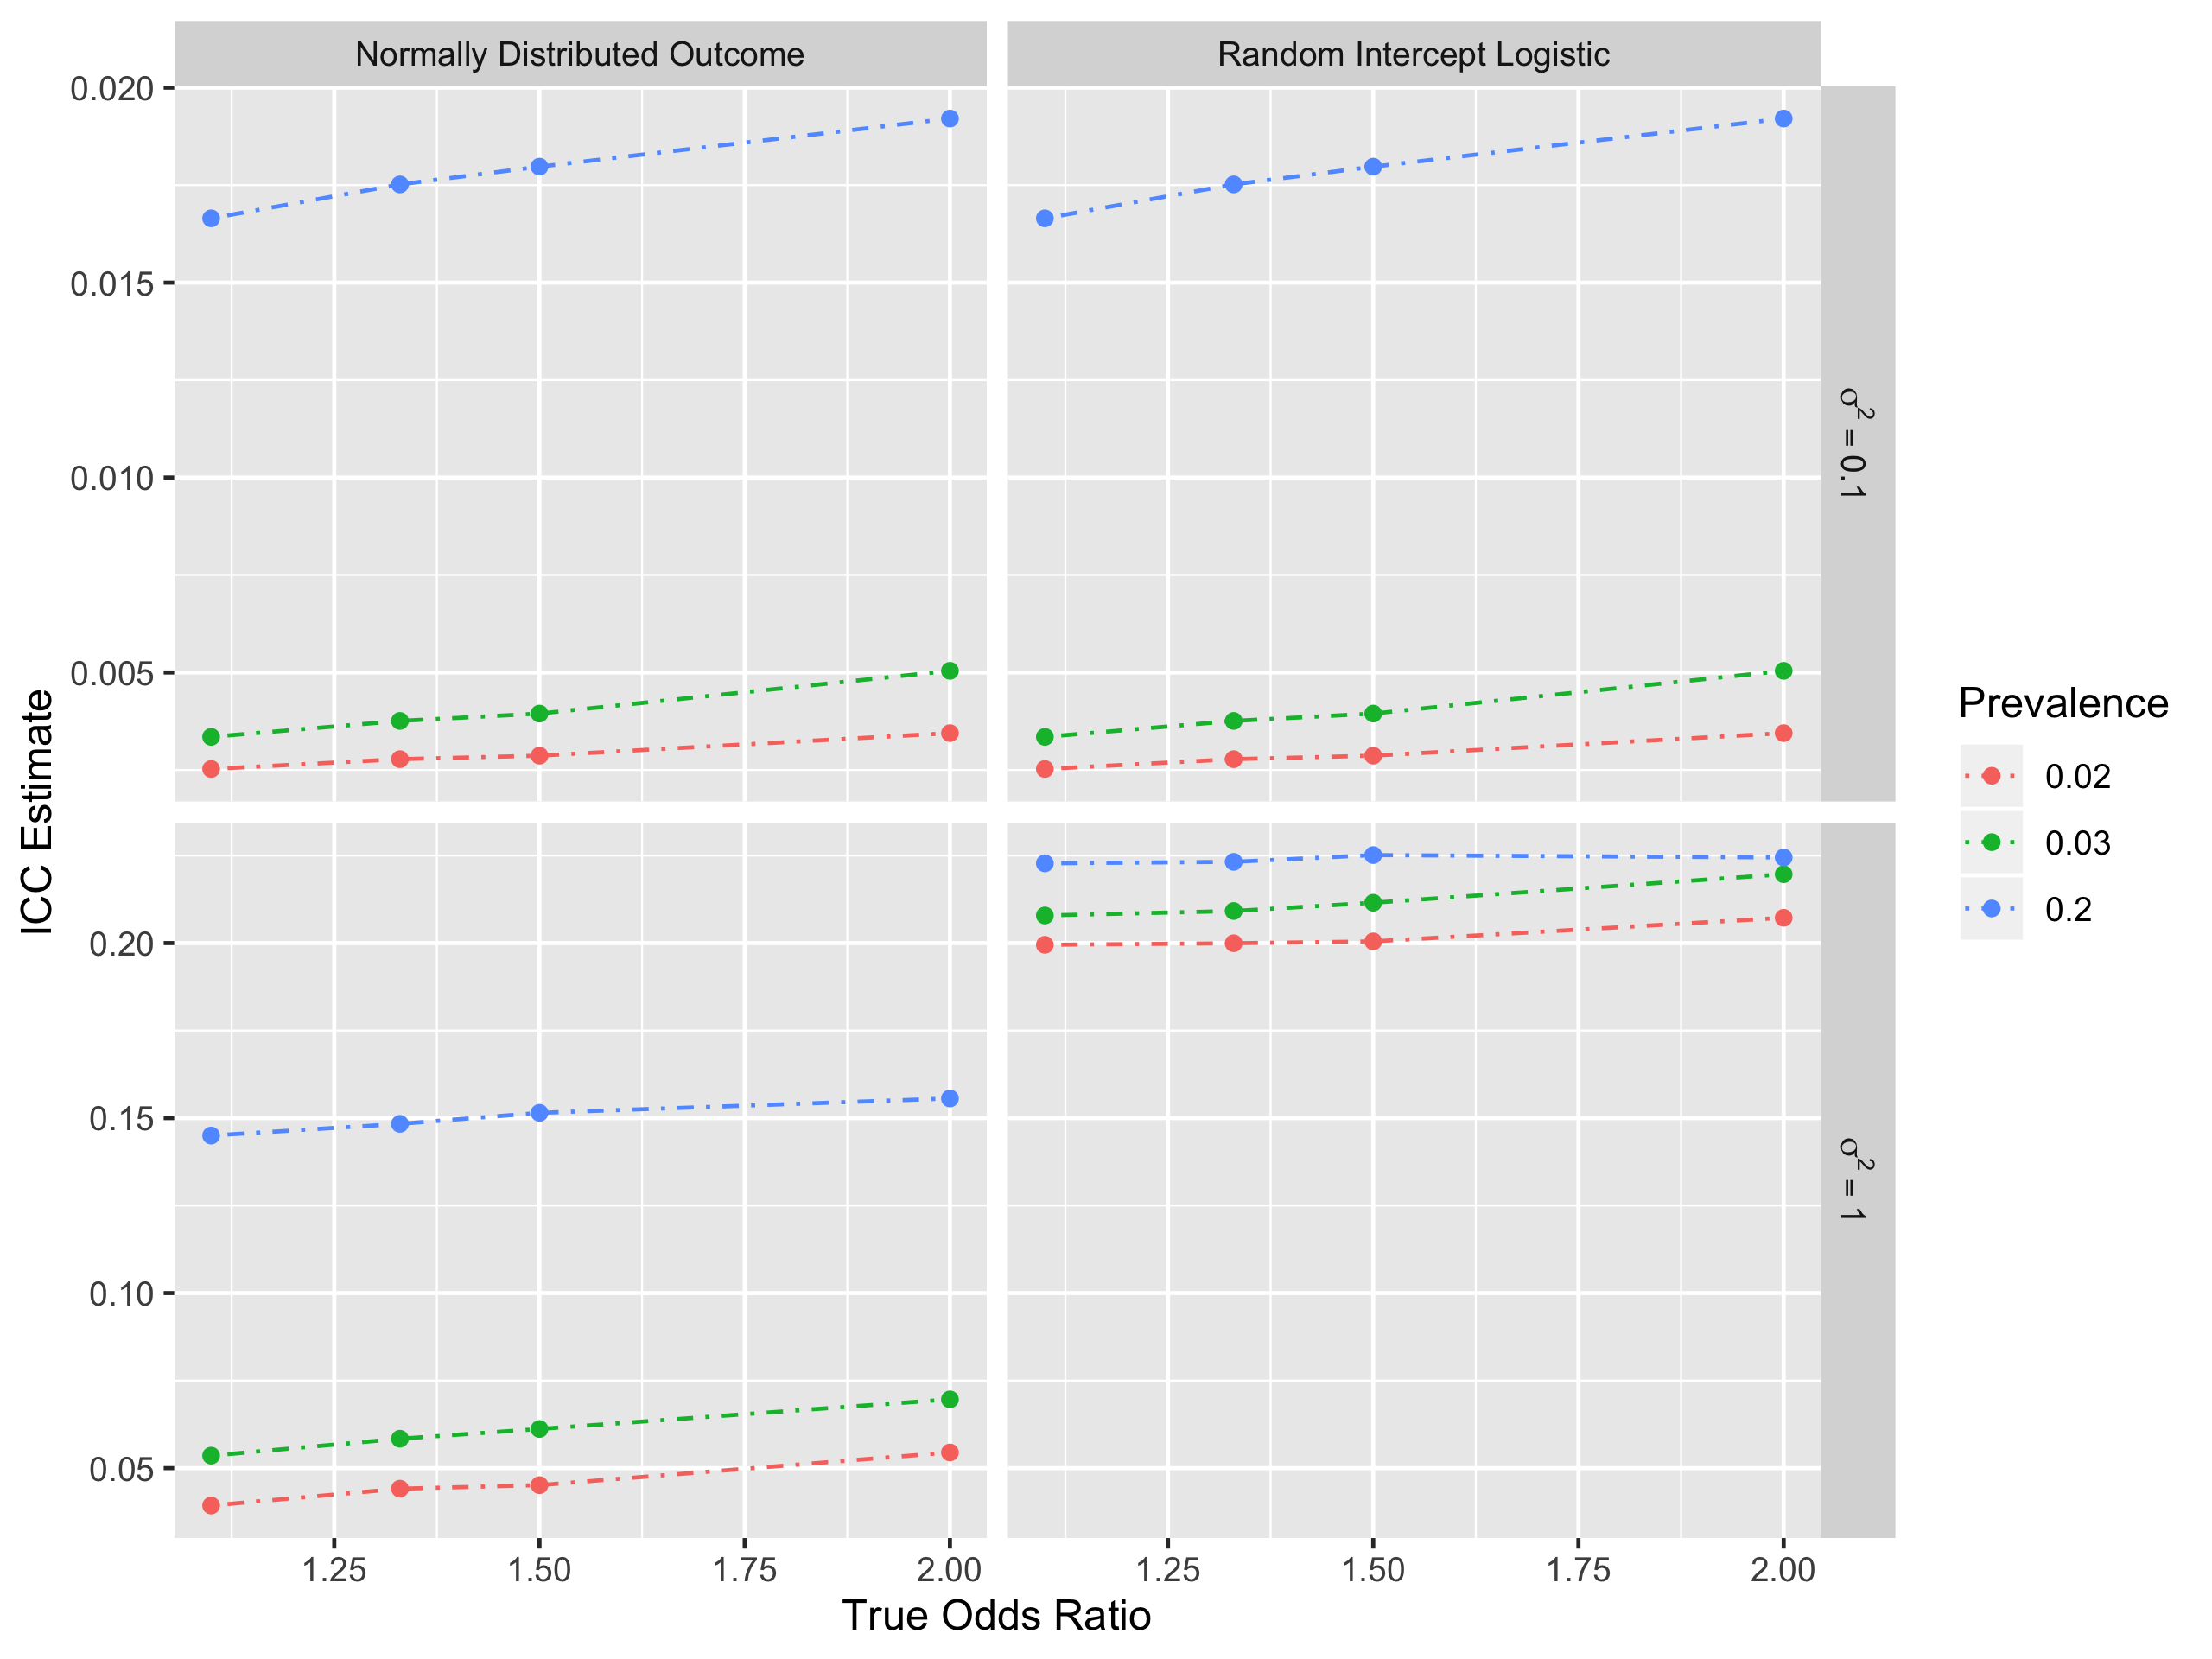
\includegraphics[width=12cm]{_icc_p100_n50.png}
  \caption{ICC estimates from models fit via PQL, $p=100$, $n=50$.}
    \label{fig:_icc}
\end{center}
\end{figure}


\section{Conclusions}

JN-- What we showed para.

JN-- What was new in what we showed.

For the vast majority of cluster randomized trials with dichotomous outcomes, GHQ is superior to PQL when fitting models. To fit a single data set with a small number of random effects, and given than most CRTs have only one random effect, the speed of GHQ with 4-10 quadrature points is adequate and it produces no detectable bias. For data analysts who are experimenting with different nested models, using Laplace approximation during the model-selection stage can save time, and GHQ can be utilized for the fitting once the final model has been chosen. Laplace is also preferable to PQL in the model-selection process because PQL only provides quasi-likelihood, and hence it is not suited to nested model comparison with the likelihood ratio test.

The bias towards the null generated by PQL is more pronounced when clusters are small, between-cluster variance is high, and baseline incidence of an outcome is low. Given our simulations, we suspect that existing studies may have suffered this bias, though it is hard to be sure given that fitting methods are rarely reported in the literature. Statisticians should report methods/functions and the algorithm options in more detail.  We should take care when selecting procedures for fitting GLMMs, particularly in SAS, where PQL is the default option. Finally, ICC estimates generated by these algorithms may vary substantially by the method used to calculate them and by the baseline prevalence of the outcome, and should be approached with a degree of skepticism.

\appendix
\section{GLMM Fitting}
Mathematically, a GLMM can be modeled as
    \begin{equation}
        g(\mu_{it})=\mathbf{x}^T_{it} \boldsymbol{\beta} + \mathbf{z}^T_{it}\mathbf{u}_i
    \end{equation}
    
    with
 $i$ a cluster indicator, $t$ an observation indicator within cluster $i$, $g$ the GLM link function, $\boldsymbol{\beta}$ a vector of coefficients for covariate values $\mathbf{x}_{it}$, and $\mathbf{z}^T_{it}$ a vector of coefficients for random effects $\mathbf{u}_i$, assumed to be distributed as multivariate normal with mean $0$ and covariance matrix $\mathbf{\Sigma}$. When the outcomes are dichotomous, the link function $g$ is typically the logit, and the mean $\mu_{it}$ is the probability of the outcome given the covariate values and cluster membership.
 
To fit a GLMM with a vector $\mathbf{x}_{it}$ and corresponding outcome vector $\mathbf{y}$, it is necessary to integrate the random effects $\mathbf{u}_i$ out of the likelihood function\cite{rodriguez_assessment_1995}. That likelihood function, the probability mass function of $y$ as a function of $\boldsymbol{\beta}$ and $\mathbf{\Sigma}$\cite{agresti_categorical_2013}, is, in general,

\begin{equation}
 \ell(\boldsymbol{\beta}, \mathbf{\Sigma} ; \mathbf{y})=f(\mathbf{y};\boldsymbol{\beta}, \mathbf{\Sigma})=\int f(\mathbf{y}|\mathbf{u};\boldsymbol{\beta})f(\mathbf{u}; \mathbf{\Sigma})d\mathbf{u}.   
\end{equation}

For many link functions of interest, including the logit link function for dichotomous outcomes considered in this paper and other situations where the response variable is discrete, the integral above does not have a closed-form solution, in part because it involves integrating the product of discrete and continuous densities\cite{ng_estimation_2006}. Numerical methods are required to approximate the integral in these circumstances.

PQL iteratively fits a linear mixed model\cite{lin_bias_1996} to the data, essentially approximating the discrete density using a Gaussian density\cite{ng_estimation_2006}. Further details of PQL have been discussed above.

Gauss-Hermite quadrature approximates the integral of a function $f(\cdot)$ multiplied by a normal density function; note that it is very similar to the likelihood function presented earlier where $f(\mathbf{u}; \mathbf{\Sigma})$ was a multivariate normal and $f(\mathbf{y}|\mathbf{u};\boldsymbol{\beta})$ the conditional likelihood. For univariate cases,

\begin{equation}
    \int_{-\infty}^{\infty}f(u)exp(-u^2)du \approx \sum_{k=1}^q c_kf(s_k)
\end{equation}

where $c_k$ are weights, sometimes from a table, and $s_k$ are the each of the quadrature points used to approximate the normal density. More quadrature points results in a more accurate approximation of the integral, but is more computationally intensive, though various GHQ subvariants have been developed that increase efficiency and reduce the number of quadrature points needed\cite{pinheiro_efficient_2006}. With GHQ, inversion of the Fisher information matrix can provide standard errors for the maximum likelihood estimates of $\boldsymbol{\beta}$ and $\mathbf{\Sigma}$. 


The Laplace method approximates the likelihood using a second-order Taylor expansion \cite{pinheiro_approximations_1995} and is is equivalent to GHQ with a single quadrature point\cite{liu_note_1994}. Simulation studies have found Laplace approximations to exhibit mild bias in coefficient estimates, and significant bias in estimation of the variance components\cite{pinheiro_efficient_2006}.

\end{flushleft}

\clearpage
\printbibliography

\end{document}
